\chapter{Model Development and Evaluation}
\section{Machine Learning Model}
Support vector machine and Multinomial NB model were trained in the training dataset given. Test dataset was used for the validation and generation of the classification report which is as follow. Multinomial NB was found to be perfoming better on test dataset with accuracy 0.58, f1-score 0.42 and weighted averate f1-score of 0.61.

\begin{figure}[H]
    \centering
    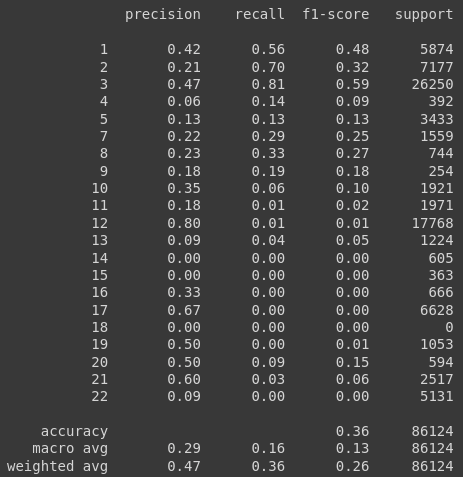
\includegraphics[scale = 0.7]{Model_cr_summary/svm_rc.png}
    \caption{SVM classification report}
    \label{fig:SVM classification report}
\end{figure}

\begin{figure}[H]
    \centering
    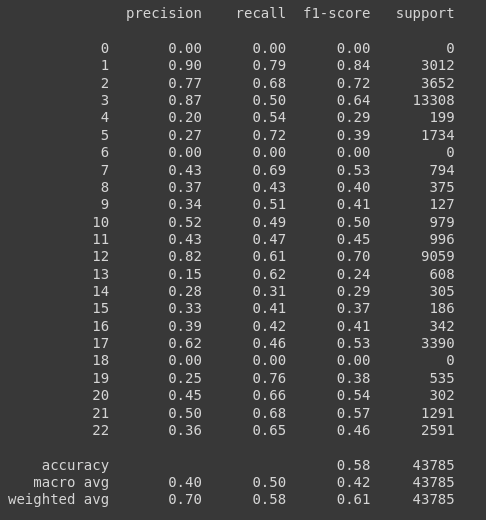
\includegraphics[scale = 0.7]{Model_cr_summary/multinomial_nb_cr.png}
    \caption{Multinomial NB classification report}
    \label{fig:Multinomial NB classification report}
\end{figure}


\section{LSTMs Dense Neural Network}
For training purpose, title and abstract of the training data were concatenated whose length distribution are shown below.

\begin{figure}[H]
    \centering
    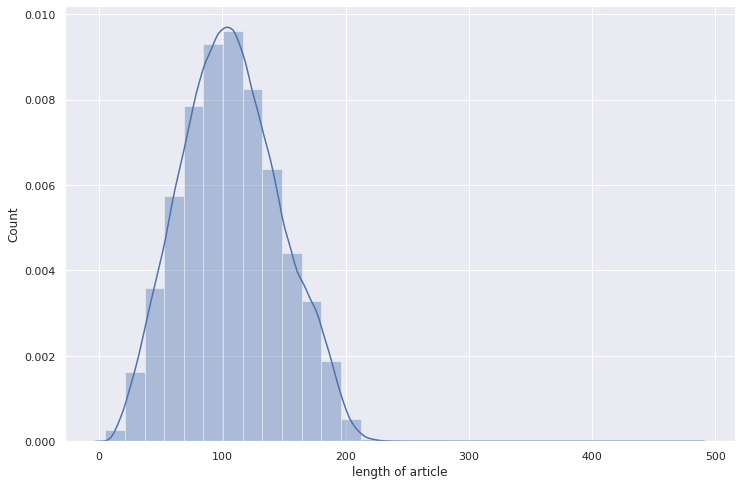
\includegraphics[scale = 0.6]{Model_cr_summary/text_length.png}
    \caption{Concatenated title and abstract length in training data}
    \label{fig:Concatenated title and abstract length in training data}
\end{figure}

From the above distribution of the text length for training data, we get the following statistics value:
\begin{table}[H]
    \begin{center}
        \begin{tabular}{ |c|c| }
            \hline
            mean               & 106.9657 \\
            \hline
            standard deviation & 39.87 \\
            \hline
            minimum            & 5       \\
            \hline
            first quartile     & 78      \\
            \hline
            median             & 105      \\
            \hline
            third quartile     & 134      \\
            \hline
            maximum            & 483     \\
            \hline
        \end{tabular}
    \end{center}
    \caption{Title and abstract length statistics based on word frequency}
    \label{table:Title and abstract length statistics based on word frequency}
\end{table}

Hence, we choose MAX\_PAD\_LENGTH = 140 for the tokenization of the data training the LSTMs Deep Neural Networks.

\subsection{LSTMs Version 1}
Any label with count less than 5000 were over-sampled to 5000 and any label with count greater than 10,000 were under-sampled to 10,000 for training in this model. The model summary and the classification report are shown below.

\begin{figure}[H]
    \centering
    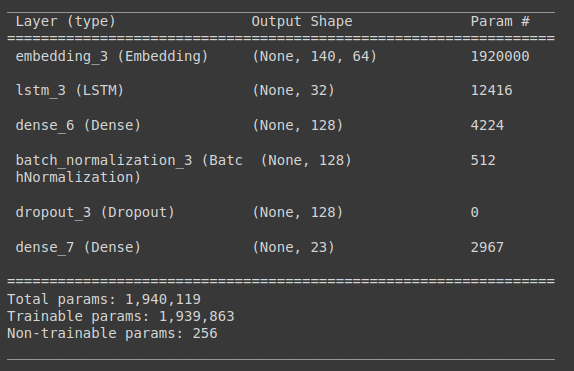
\includegraphics[scale = 0.7]{Model_cr_summary/sequential_v1_model.png}
    \caption{Model summary for version 1}
    \label{fig:Model summary for version 1}
\end{figure}

\begin{figure}[H]
    \centering
    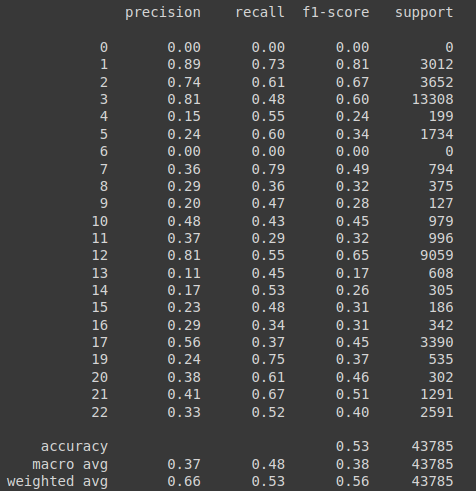
\includegraphics[scale = 0.7]{Model_cr_summary/sequential_v1_cr.png}
    \caption{Classification report for Version 1}
    \label{fig: Classification report for Version 1}
\end{figure}

\subsection{LSTMs Version 2}
The model was same as in the Version 1. However, no. of LSTMs unit was reduced from 32 to 10 in this version and the result obtained were as follow. We can observe that the test accuracy improves from 0.53 to 0.68, macro average F1-score from 0.38 to 0.45.

\begin{figure}[H]
    \centering
    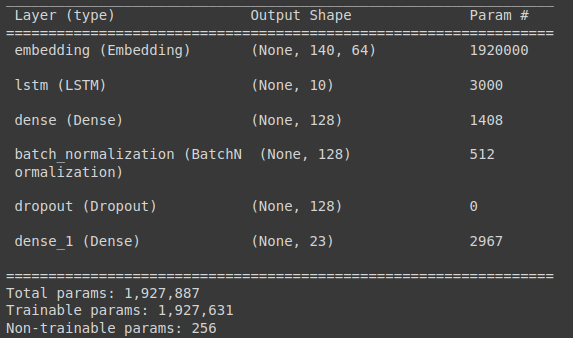
\includegraphics[scale = 0.7]{Model_cr_summary/sequential_v4_model.png}
    \caption{Model summary for version 2}
    \label{fig:Model summary for version 2}
\end{figure}

\begin{figure}[H]
    \centering
    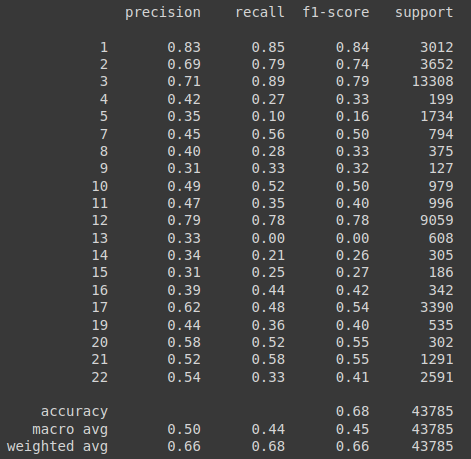
\includegraphics[scale = 0.6]{Model_cr_summary/sequential_v4_cr.png}
    \caption{Classification report for Version 2}
    \label{fig: Classification report for Version 2}
\end{figure}

The graph regarding loss, accuracy, f1-score and fbeta-score are as follow:

\begin{figure}[H]
    \centering
    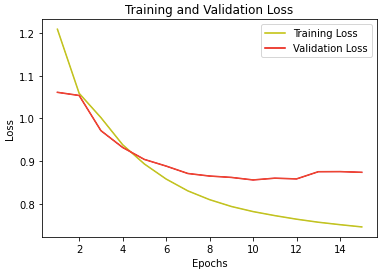
\includegraphics[scale = 0.6]{training_testing/seq_v4_loss.png}
    \caption{LSTMs V2 Loss curve}
    \label{fig:LSTMs V2 loss curve}
\end{figure}

\begin{figure}[H]
    \centering
    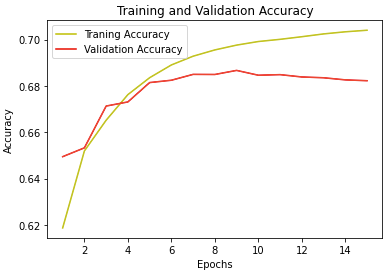
\includegraphics[scale = 0.6]{training_testing/seq_v4_accuracy.png}
    \caption{LSTMs V2 accuracy curve}
    \label{fig:LSTMs V2 accuracy curve}
\end{figure}

\begin{figure}[H]
    \centering
    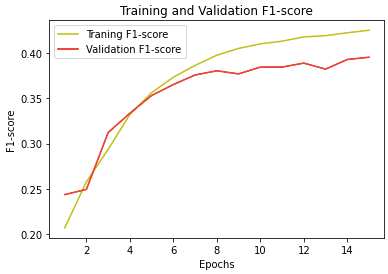
\includegraphics[scale = 0.6]{training_testing/seq_v4_f1.png}
    \caption{LSTMs V2 F1-score curve}
    \label{fig:LSTMs V2 F1-score curve}
\end{figure}

\begin{figure}[H]
    \centering
    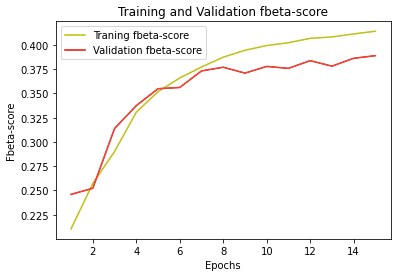
\includegraphics[scale = 0.6]{training_testing/seq_v4_beta.png}
    \caption{LSTMs V2 fbeta-score curve}
    \label{fig:LSTMs V2 fbeta-score curve}
\end{figure}

\section{Transformer Model}
For the test data while training transformer model, we observed that the 32,404 rows in test data are duplicates of the training data. Hence We removed those rows from the test data for creating the classification report.

\subsection{Transformer Version 1}
We can observe form the classification report that the accuracy improves to 0.69 and macro average f1-score to 0.46.

\begin{figure}[H]
    \centering
    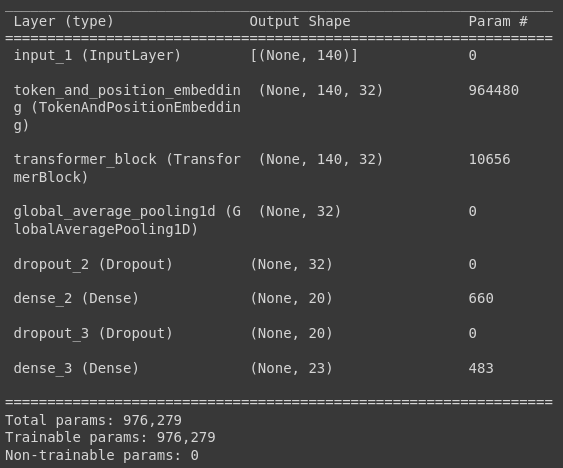
\includegraphics[scale = 0.55]{Model_cr_summary/transformer_v1_model.png}
    \caption{Transformer Model summary for version 1}
    \label{fig:Transformer Model summary for version 1}
\end{figure}

\begin{figure}[H]
    \centering
    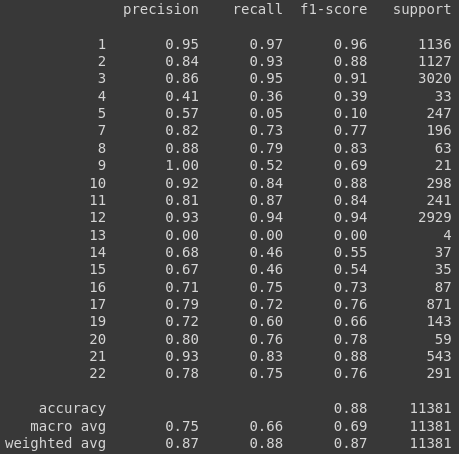
\includegraphics[scale = 0.6]{Model_cr_summary/transformer_v1_cr_no_rep.png}
    \caption{Transformer Classification report for Version 1}
    \label{fig:Transformer Classification report for Version 1}
\end{figure}

The graph regarding loss, accuracy, f1-score and fbeta-score are as follow:

\begin{figure}[H]
    \centering
    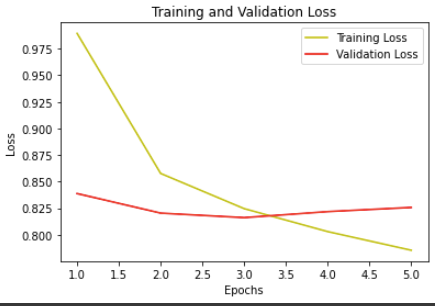
\includegraphics[scale = 0.6]{training_testing/transformer_v1_loss.png}
    \caption{Transformer V1 Loss curve}
    \label{fig:Transformer V1 loss curve}
\end{figure}

\begin{figure}[H]
    \centering
    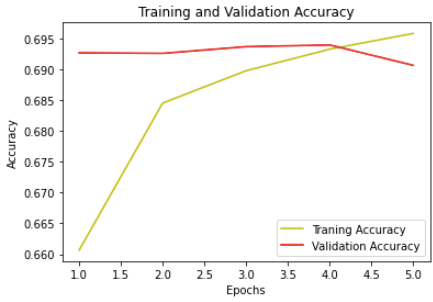
\includegraphics[scale = 0.6]{training_testing/transformer_v1_accuracy.png}
    \caption{Transformer V1 accuracy curve}
    \label{fig:Transformer V1 accuracy curve}
\end{figure}

\begin{figure}[H]
    \centering
    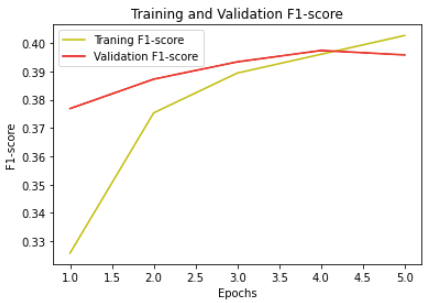
\includegraphics[scale = 0.6]{training_testing/transformer_v1_f1.png}
    \caption{Transformer F1-score curve}
    \label{fig:Transformer F1-score curve}
\end{figure}

\begin{figure}[H]
    \centering
    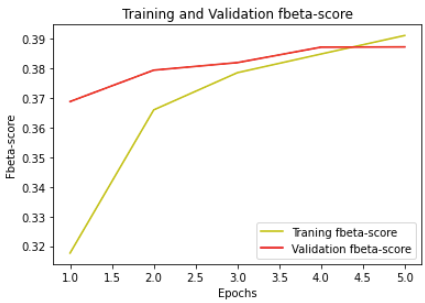
\includegraphics[scale = 0.6]{training_testing/transformer_v1_beta.png}
    \caption{Transformer V1 fbeta-score curve}
    \label{fig:Transformer V1 fbeta-score curve}
\end{figure}

\subsection{Transformer Version 2}
The model summary was same as in transformer version 1. However, for training this model, we oversampled the label with count less than 1000 to 1000 and provided class weights using sklearn.utils.class$\_$weights. The classification report and model history curve are as follow:

\begin{figure}[H]
    \centering
    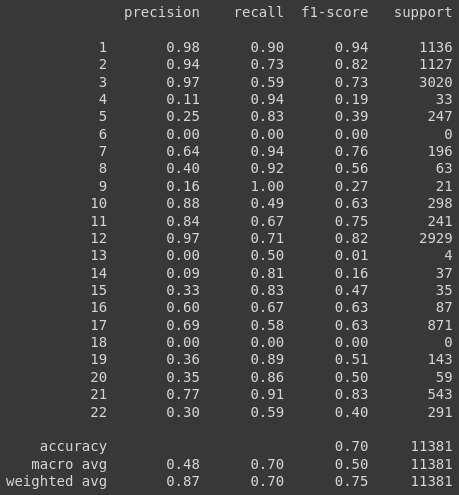
\includegraphics[scale = 0.55]{Model_cr_summary/transformer_v2_cr.png}
    \caption{Transformer Classification report for version 2}
    \label{fig:Transformer Classification report for version 2}
\end{figure}

\begin{figure}[H]
    \centering
    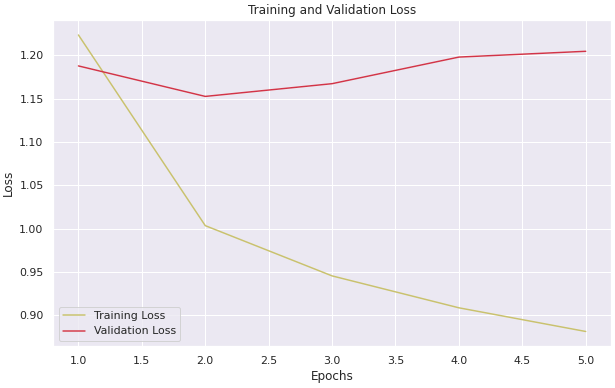
\includegraphics[scale = 0.6]{training_testing/transformer_v2_loss.png}
    \caption{Transformer V2 Loss curve}
    \label{fig:Transformer V2 loss curve}
\end{figure}

\begin{figure}[H]
    \centering
    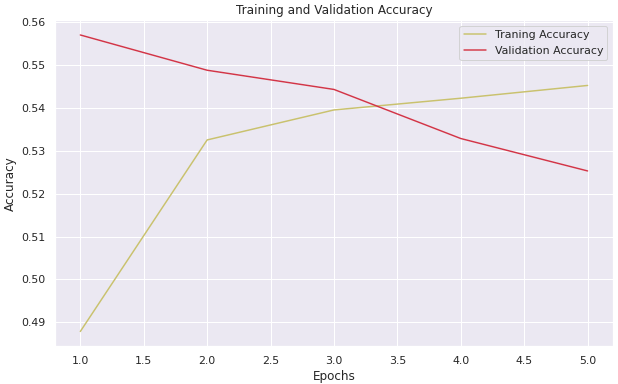
\includegraphics[scale = 0.6]{training_testing/transformer_v2_accuracy.png}
    \caption{Transformer V2 accuracy curve}
    \label{fig:Transformer V2 accuracy curve}
\end{figure}

\begin{figure}[H]
    \centering
    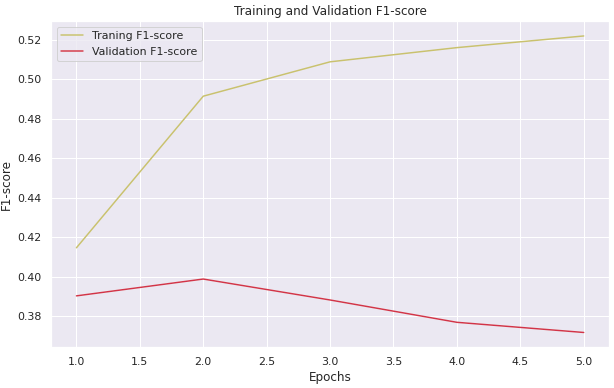
\includegraphics[scale = 0.6]{training_testing/transformer_v2_f1.png}
    \caption{Transformer F2-score curve}
    \label{fig:Transformer F2-score curve}
\end{figure}

\begin{figure}[H]
    \centering
    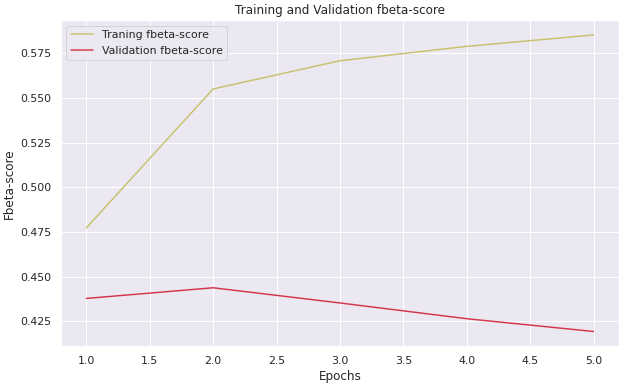
\includegraphics[scale = 0.6]{training_testing/transformer_v2_beta.png}
    \caption{Transformer V2 fbeta-score curve}
    \label{fig:Transformer V2 fbeta-score curve}
\end{figure}

\subsection{Pretrained BERT Model}
For Bert, the pretrained model was taken from hugging face transformers. The sentences were tokenized using pretrained bert tokenizer.
The pretrained encoding from model was taken, on top of which 3 layerd 
multi-layered 
perceptron of layer$\_$size 
= (480,360,180) 
was used with dropout layer(p = 0.1). The classification report was as follow:

\begin{figure}[H]
    \centering
    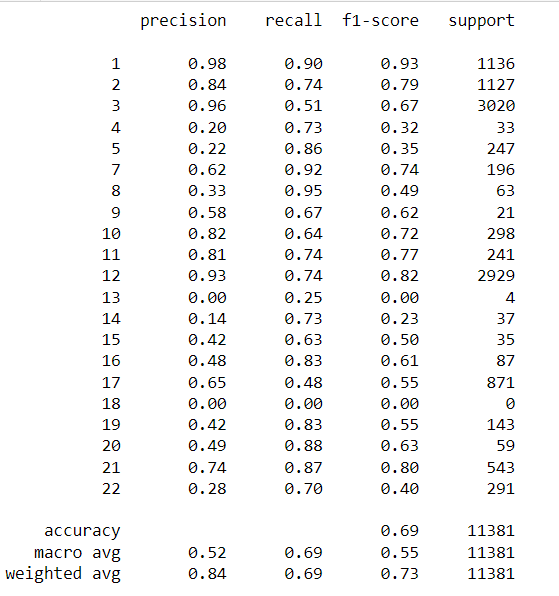
\includegraphics[scale = 0.45]{Model_cr_summary/bert_cr.png}
    \caption{Bert Classification Report}
    \label{fig:Bert Model Classification Report}
\end{figure}

\section{Model Comparision}
\begin{table}[H]
    \begin{center}
        \begin{tabular}{ |c|c|c|c| }
            \hline
            Model Name               & Accuracy & Macro Average & Weighted Average \\
            \hline
            Multinomial NB & 0.58 & 0.42 & 0.61\\
            \hline
            SVM            & 0.36       & 0.13 & 0.26\\
            \hline
            LSTMs V1    & 0.53      & 0.38 & 0.56\\
            \hline
            LSTMs V2    & 0.68  & 0.45 & 0.66\\
            \hline
            Transformer V1     & .88  & .69 & .87 \\
            \hline
            Transformer V2   &   .70   & .50 & .75 \\
            \hline
            BERT  &   .69   & .55 & .73 \\
            \hline
        \end{tabular}
    \end{center}
    \caption{Model Comparision based on classification report}
    \label{table:Model Comparision based on classification report}
\end{table}

From the table \ref{table:Model Comparision based on classification report}, we found that transformer V1 is better than the transformer V2 and LSTMs V2 is better than LSTMs V1.

In both LSTMs V1 and transformer V2, we did sampling and provided class weights for correcting the class imbalance. However the result was not good. This is because, the test data provided itself was highly imbalanced and biased toward the majority class as in training data which we can observe from the support column of the classification report. Hence, we got better accuracy and f1-score in the model when no sampling and class weights are provided as in the LSTMs V2 and transformer V1. 

However, if the test data would have contained minority classes data too, then the result could change. 

